\newcommand{\TabTgtImprovDiskParams}{
\begin{table}[tb]
\centering
\sisetup{
table-number-alignment=center
}
\begin{tabular}{|r|S[table-format=5.1]S[table-format=1.5]S[table-format=3.3]|}
\multicolumn{1}{|L{1.1cm}}{Disk Index} & \multicolumn{1}{|L{1.8cm}}{Beamline Position (mm)} & \multicolumn{1}{L{1.5cm}}{Relative Gyroradius} & \multicolumn{1}{L{2cm}|}{Disk Radius in Simulation} \\
\hline
0 & 19542.0 & 1.09832 & 144.758 \\
1& 19592.1 & 1.11405 & 148.932 \\
2& 19642.2 & 1.13064 & 153.400 \\
3& 19692.3 & 1.14836 & 158.248 \\
4& 19742.4 & 1.16753 & 163.576 \\
5& 19792.5 & 1.18847 & 169.495 \\
6& 19842.6 & 1.21130 & 176.068 \\
7& 19892.7 & 1.23601 & 183.326 \\
8& 19942.8 & 1.26227 & 191.198 \\
9& 19992.9 & 1.28943 & 199.516 \\
10 & 20043.0 & 1.31668 & 208.037 \\
11 & 20093.1 & 1.34304 & 216.451 \\
12 & 20143.2 & 1.36771 & 224.474 \\
13 & 20193.3 & 1.39005 & 231.867 \\
14 & 20243.4 & 1.40984 & 238.518 \\
15 & 20293.5 & 1.42688 & 244.317 \\
16 & 20343.6 & 1.44127 & 249.272 \\
17 & 20393.7 & 1.45330 & 253.450 \\
\hline
\end{tabular}~%
\begin{tabular}{|r|S[table-format=5.1]S[table-format=1.5]S[table-format=3.3]|}
\multicolumn{1}{|L{1.1cm}}{Disk Index} & \multicolumn{1}{|L{1.8cm}}{Beamline Position (mm)} & \multicolumn{1}{L{1.5cm}}{Relative Gyroradius} & \multicolumn{1}{L{2cm}|}{Disk Radius in Simulation} \\
\hline
18 & 20443.8 & 1.46330 & 256.950 \\
19 & 20493.9 & 1.47151 & 259.842 \\
20 & 20544.0 & 1.47823 & 262.219 \\
21 & 20594.1 & 1.48347 & 264.080 \\
22 & 20644.2 & 1.48745 & 265.500 \\
23 & 20694.3 & 1.49056 & 266.612 \\
24 & 20744.4 & 1.49296 & 267.471 \\
25 & 20794.5 & 1.49478 & 268.125 \\
26 & 20844.6 & 1.49612 & 268.604 \\
27 & 20894.7 & 1.49703 & 268.933 \\
28 & 20944.8 & 1.49730 & 269.030 \\
29 & 20994.9 & 1.49730 & 269.030 \\
30 & 21045.0 & 1.49714 & 268.972 \\
31 & 21095.1 & 1.49692 & 268.891 \\
32 & 21145.2 & 1.49671 & 268.817 \\
33 & 21195.3 & 1.49667 & 268.804 \\
34 & 21245.4 & 1.49673 & 268.823 \\
   &         &         &         \\
\hline
\end{tabular}
\caption{
Parameters of the target disks used in the proof of principle simulation.
Since the beamline axis is parallel to the $-z$ direction in the stopping target region, the Z-coordinate can be obtained from the beamline position via: $z=2164-(s-19542)$.
\tablabel{app:tgtImprov:diskParams}}
\end{table}
}

\newcommand{\FigTgtImprovFieldVsBeamline}{
\begin{figure}[tb]
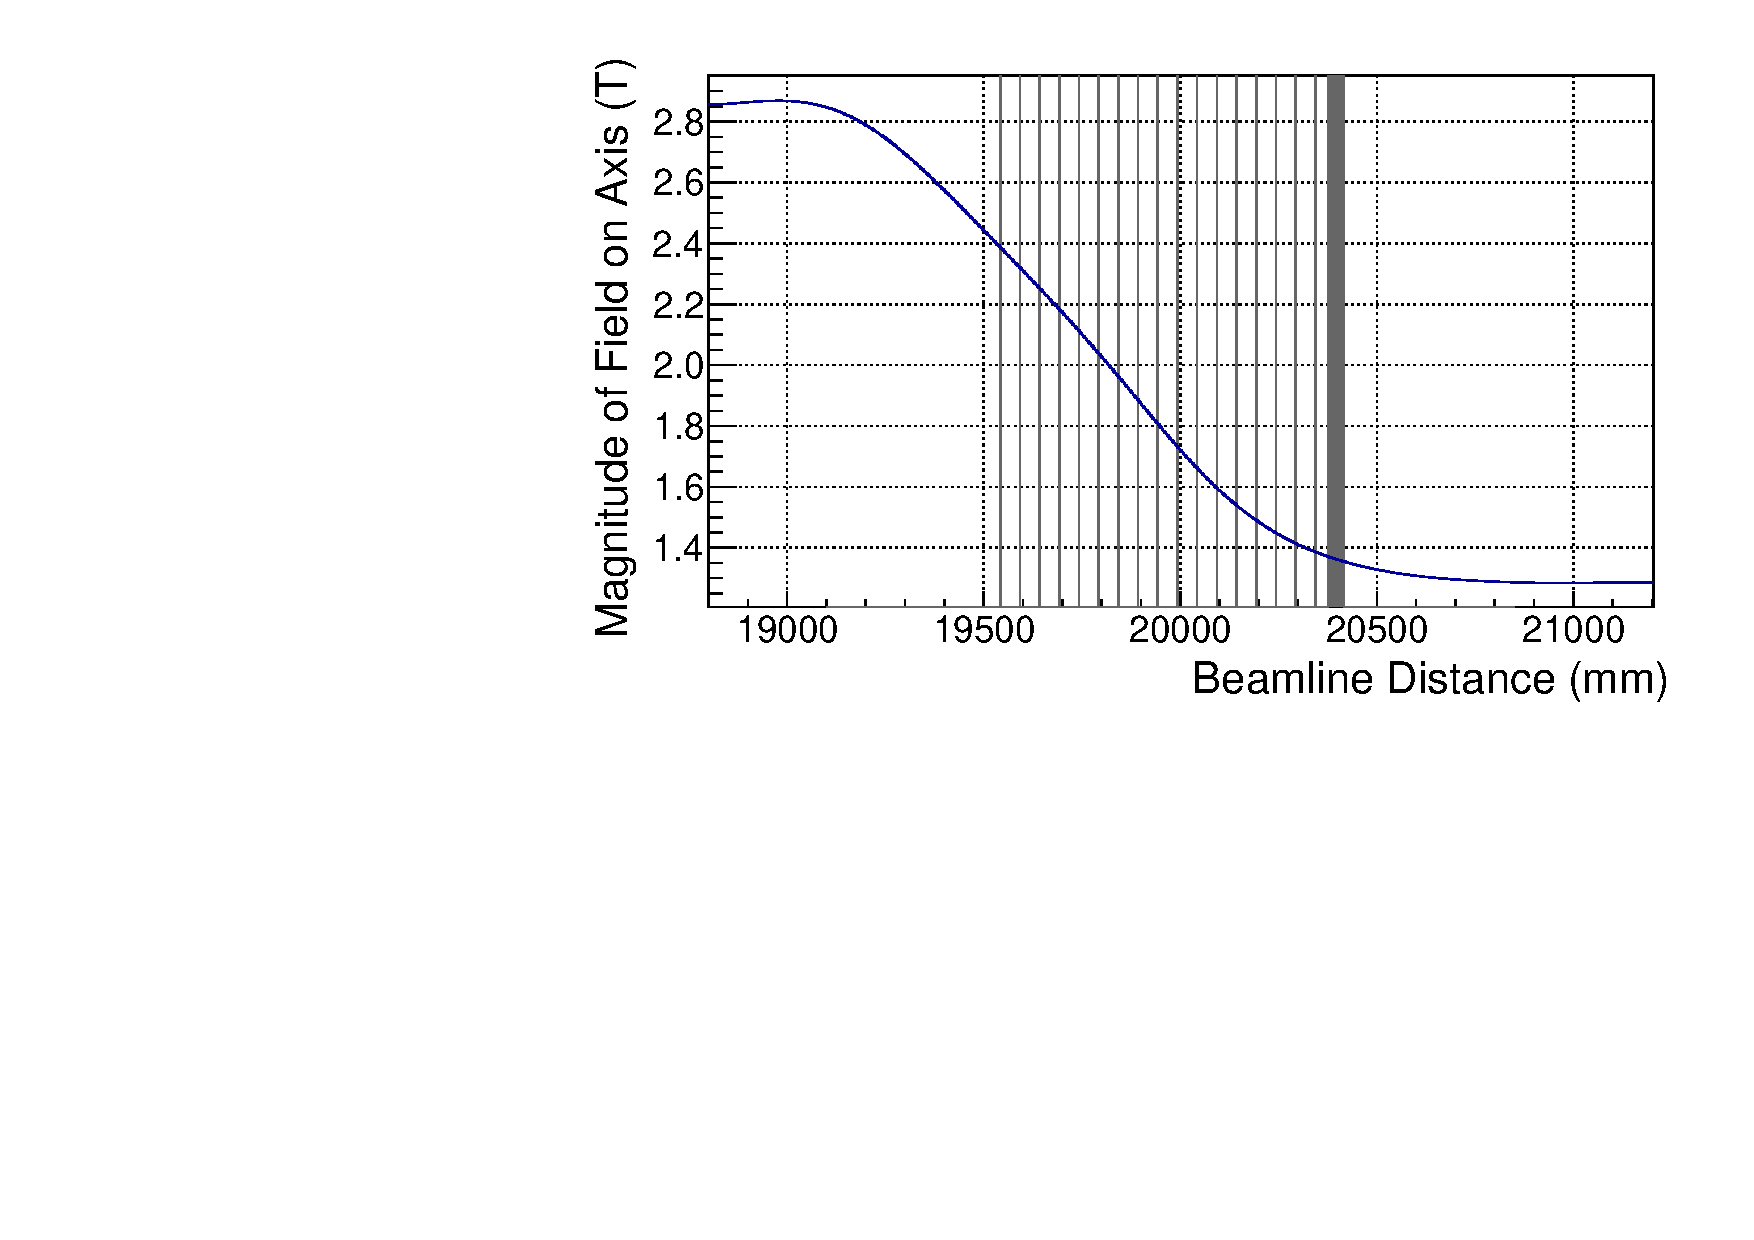
\includegraphics[width=0.9\textwidth,trim=1.0cm 0cm 0.8cm 0,clip]{figs/appendixStopTgtImprov/Plot_FieldMagnitude.pdf}
\caption{
The magnitude of the magnetic field around the stopping target.
The vertical grey lines indicate the position of the stopping target disks and beam blocker in the target design used in chapter~\sect{sense}.
The muon beam arrives from the left, and signal electrons should leave to the right.
\figlabel{app:tgtImprov:field}}
\end{figure}
}

\newcommand{\FigTgtImprovMirrorVsBeamline}{
\begin{figure}[tb]
\subfloat[][\figlabel{app:tgtImprov:mirror:thetaMin}Minimum Pitch Angle]{%
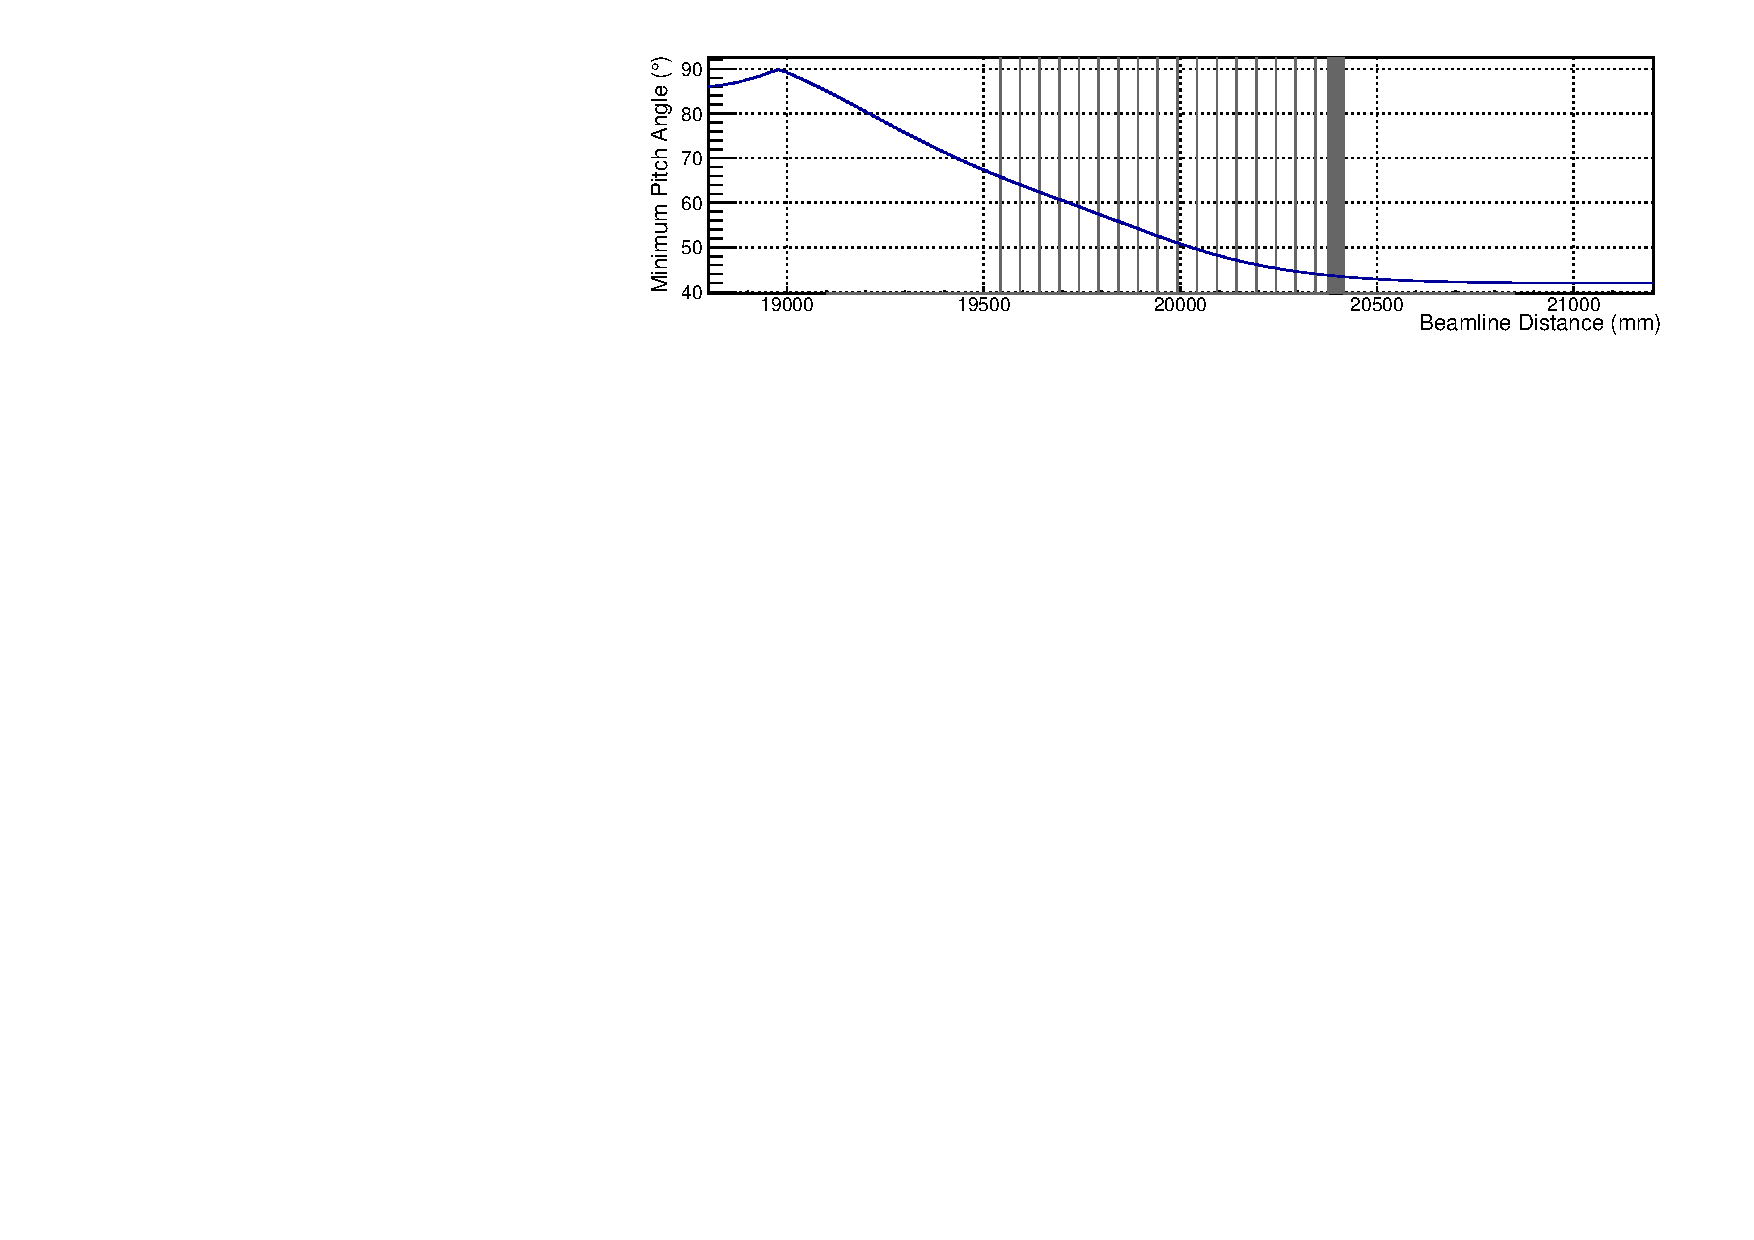
\includegraphics[width=0.9\textwidth,trim=1.5cm 0 0.8cm 0,clip]{figs/appendixStopTgtImprov/Plot_ThetaMin.pdf}}\\
\subfloat[][\figlabel{app:tgtImprov:mirror:phaseSpace}Fraction of Space Which Can be Mirrored]{%
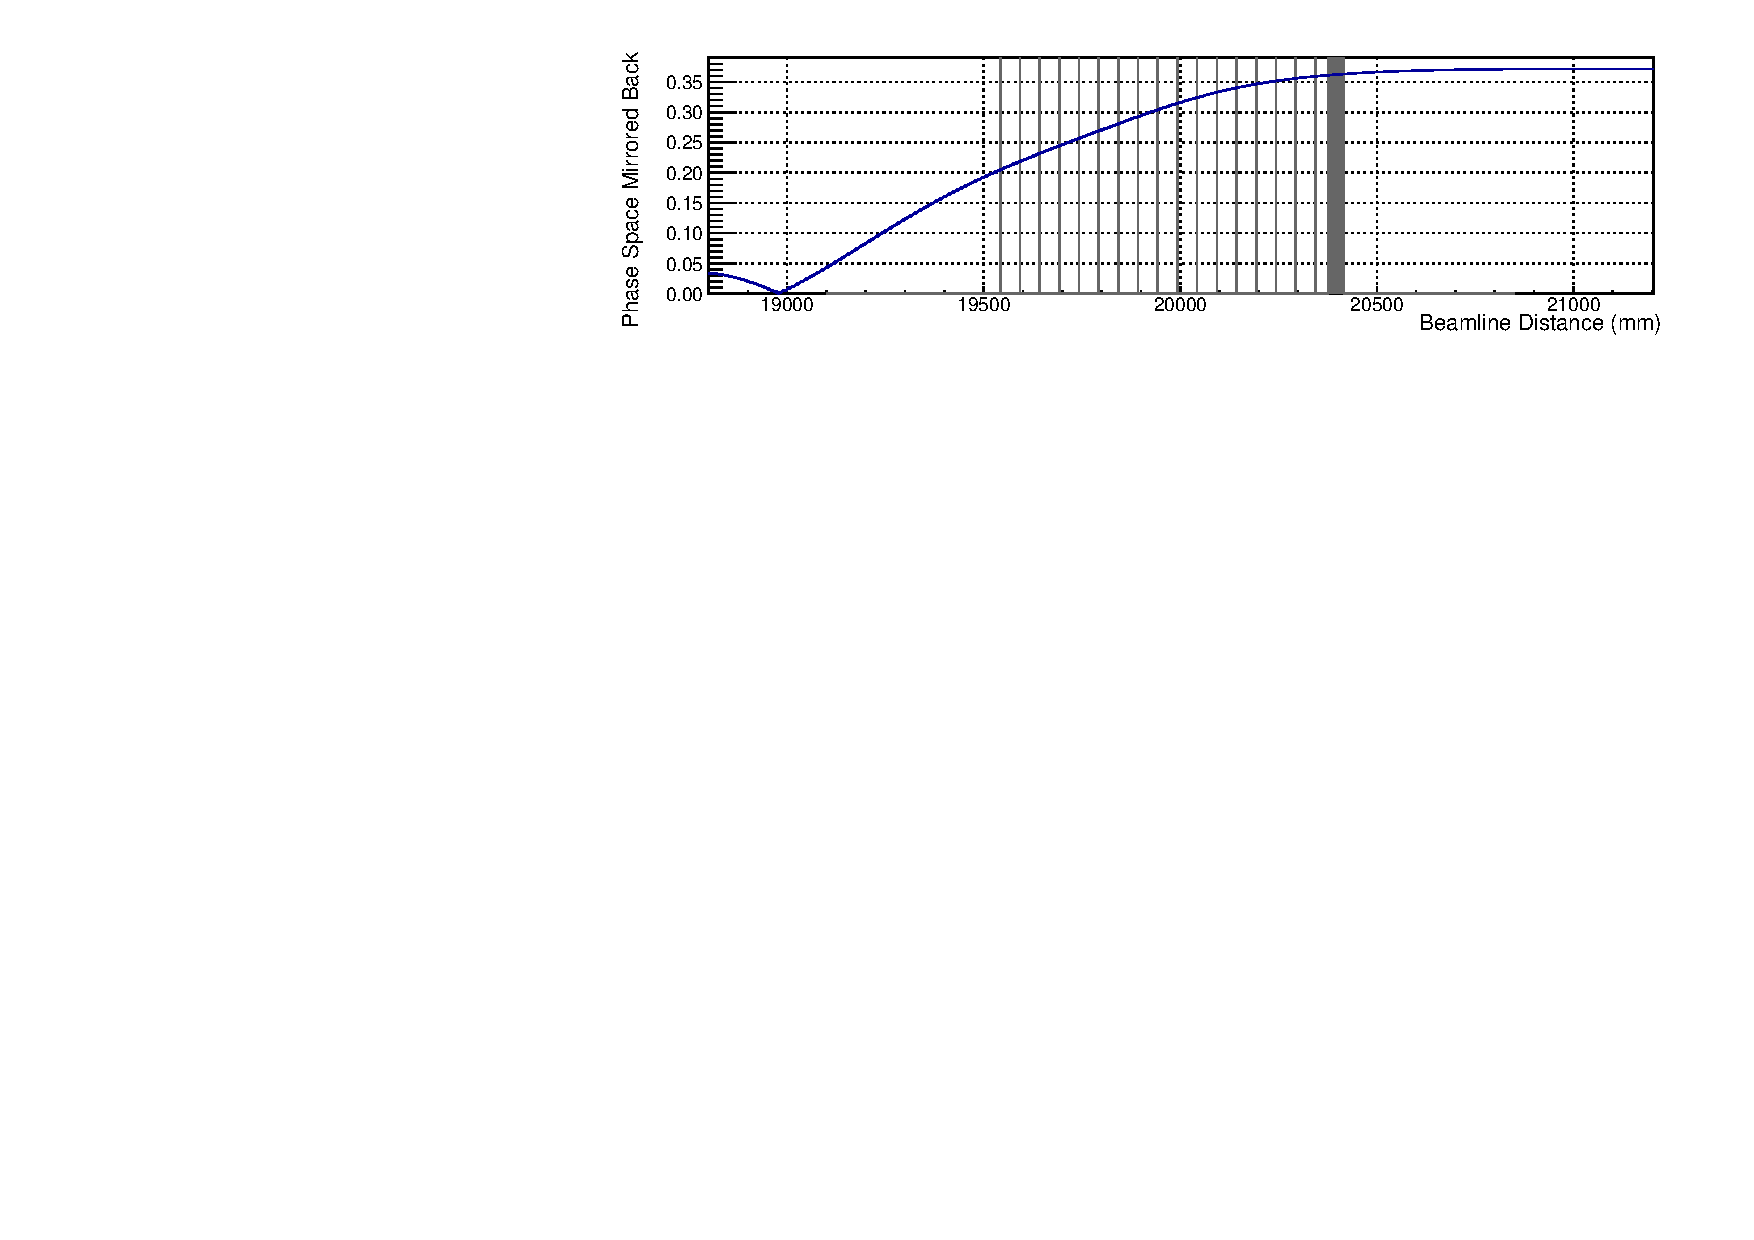
\includegraphics[width=0.9\textwidth,trim=1.5cm 0 0.8cm 0,clip]{figs/appendixStopTgtImprov/Plot_PhaseSpaceFraction.pdf}}
\caption{
The ability for a particle to be mirrored downstream, if it is initially heading upstream at this point.
For an electron produced at a given point along the beamline, if its pitch angle is too small it will not be mirrored.
The minimum pitch angle is shown in \protect\subref{fig:app:tgtImprov:mirror:thetaMin}.
Since electrons are produced isotropically, this minimum pitch angle can be used to define the fraction of phase space that will be mirrored back, \protect\subref{fig:app:tgtImprov:mirror:phaseSpace}.
\figlabel{app:tgtImprov:mirror}}
\end{figure}
}

\newcommand{\FigTgtImprovGyroradiusVsBeamline}{
\begin{figure}[tb]
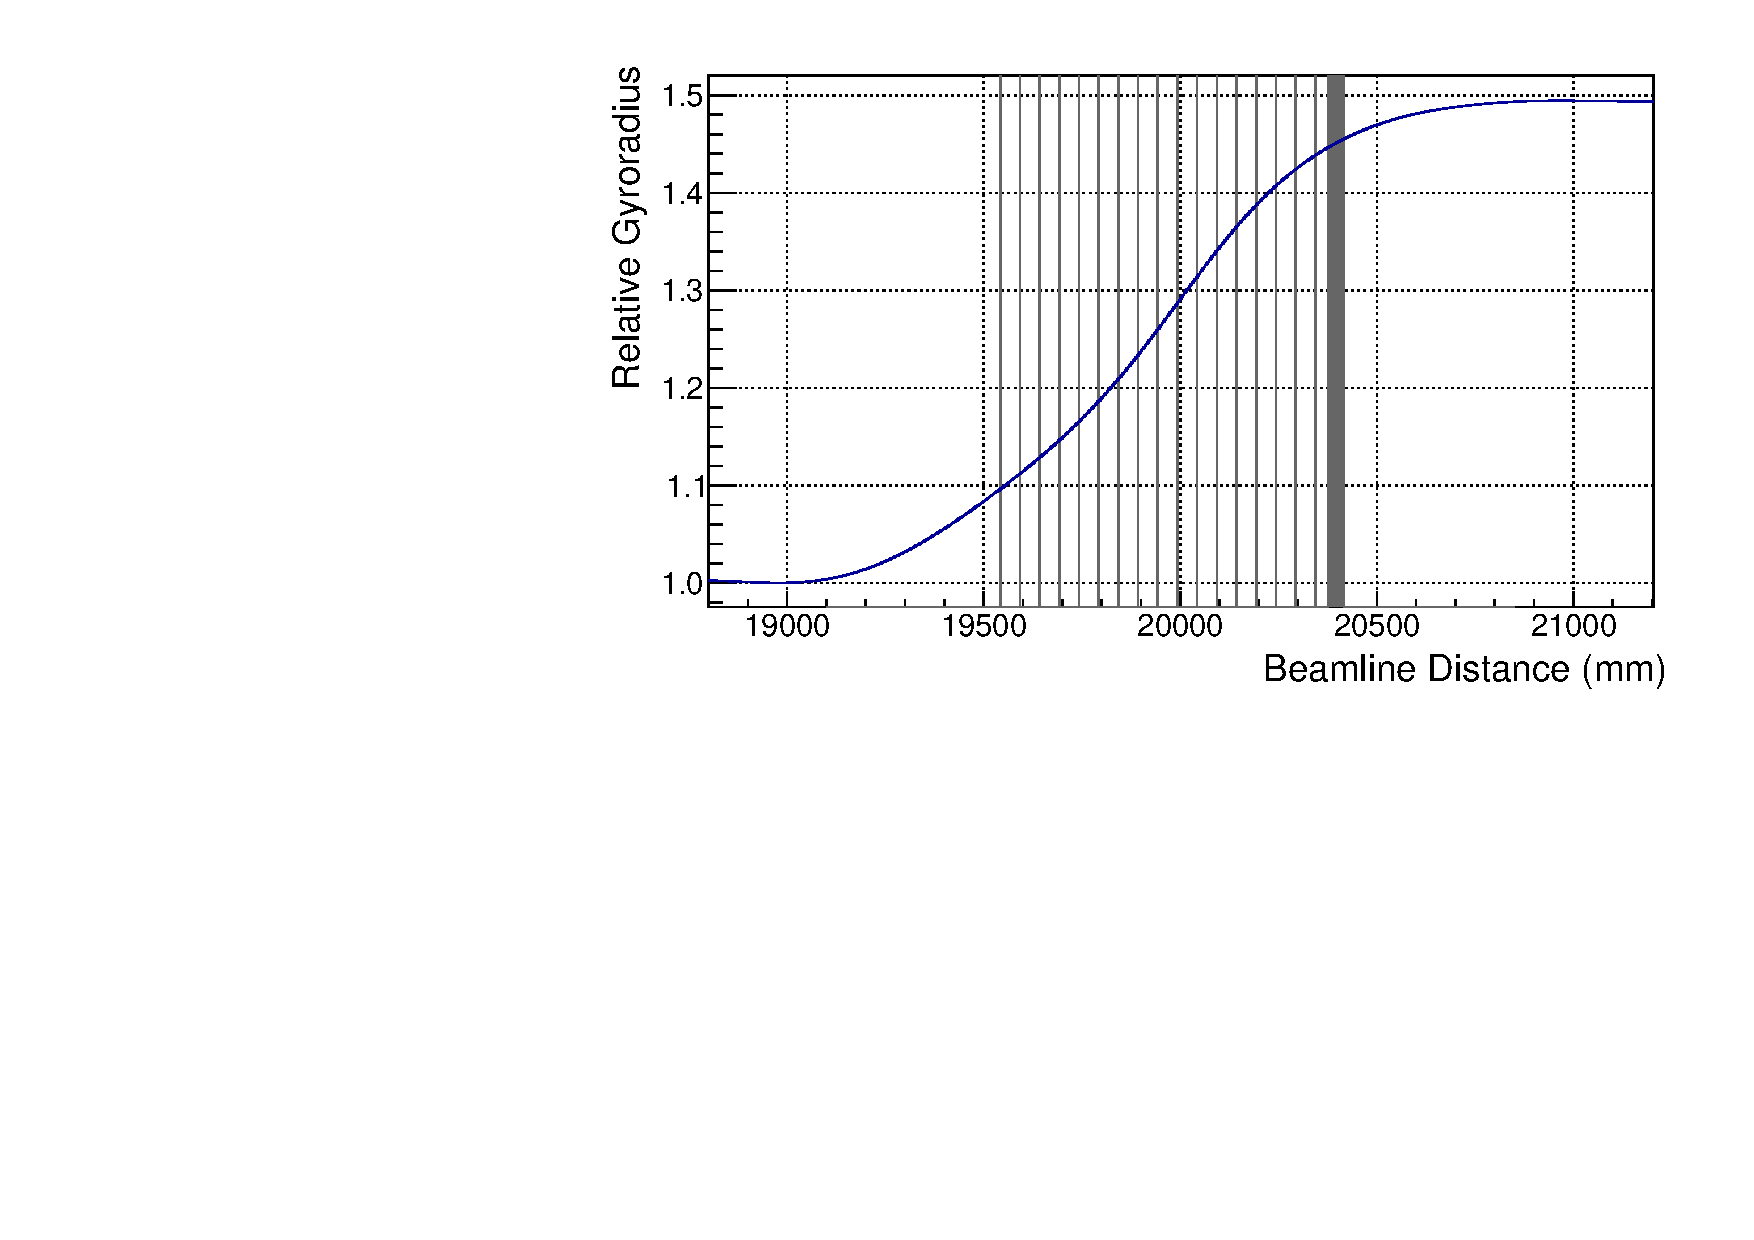
\includegraphics[width=0.9\textwidth,trim=1.2cm 0.2cm 0.8cm 0.2cm,clip]{figs/appendixStopTgtImprov/Plot_GyroradiusGrowth.pdf}
\caption{
As the muon beam progresses along the beamline, the beam envelope varies proportional to the square root of the field strength.
The maximum field occurs at the exit of the Torus2 solenoid, with a field strength of about 2.88~T, and this plot shows the relative change in the beam envelope compared to that point.
\figlabel{app:tgtImprov:gyroradius}}
\end{figure}
}

\newcommand{\FigTgtImprovSenseVsBeamline}{
\begin{figure}[tb]
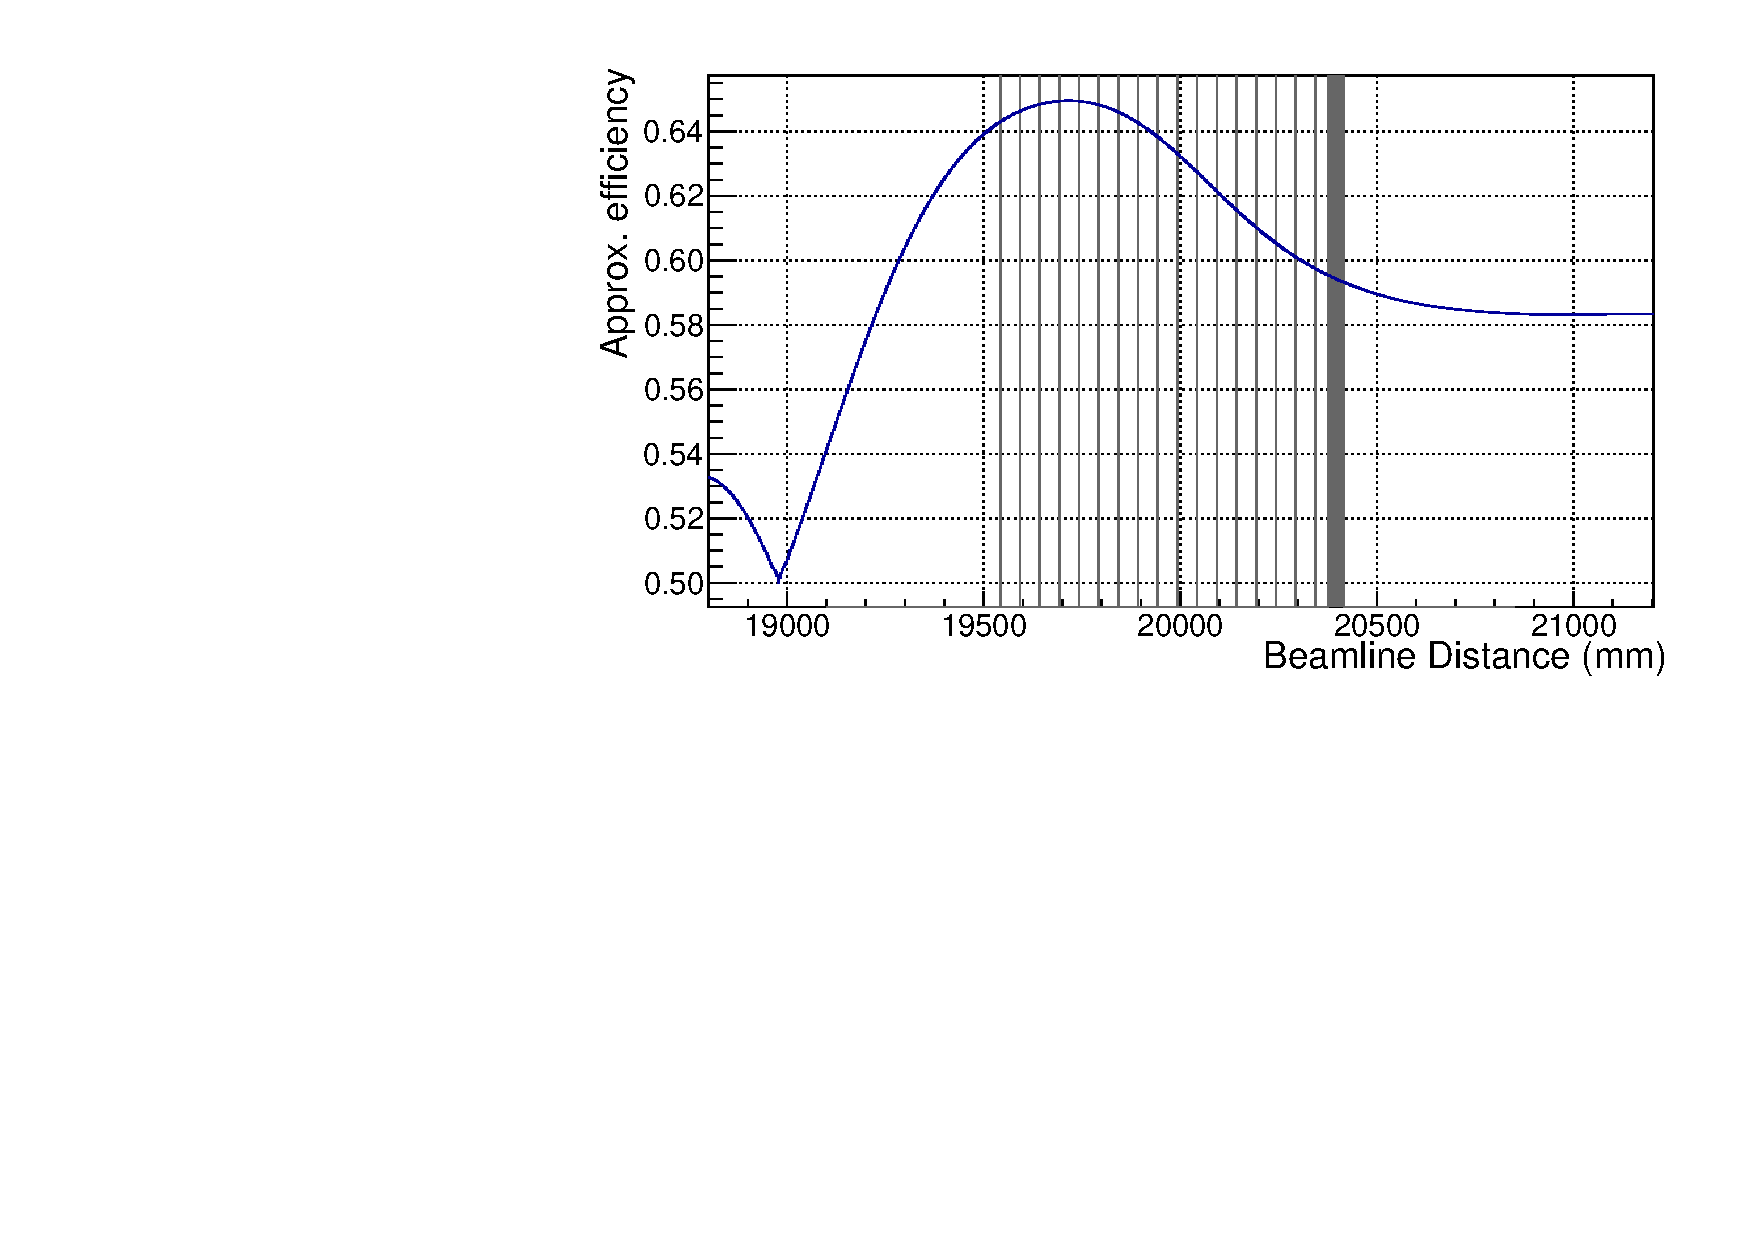
\includegraphics[width=0.9\textwidth,trim=1.1cm 0.3cm 0.8cm 0.3cm,clip]{figs/appendixStopTgtImprov/Plot_ApproxEfficiency.pdf}
\caption{
The effective signal sensitivity achieved by placing a disk of fixed radius at a given location along the beamline.
It suggests an optimal target position slightly upstream of the location found in the optimisation chapter, but the difference is easily explained by simplifications in this model.
\figlabel{app:tgtImprov:senseVsBeamline}}
\end{figure}
}

\newcommand{\FigTgtImprovNewGeom}{
\begin{figure}[tb]
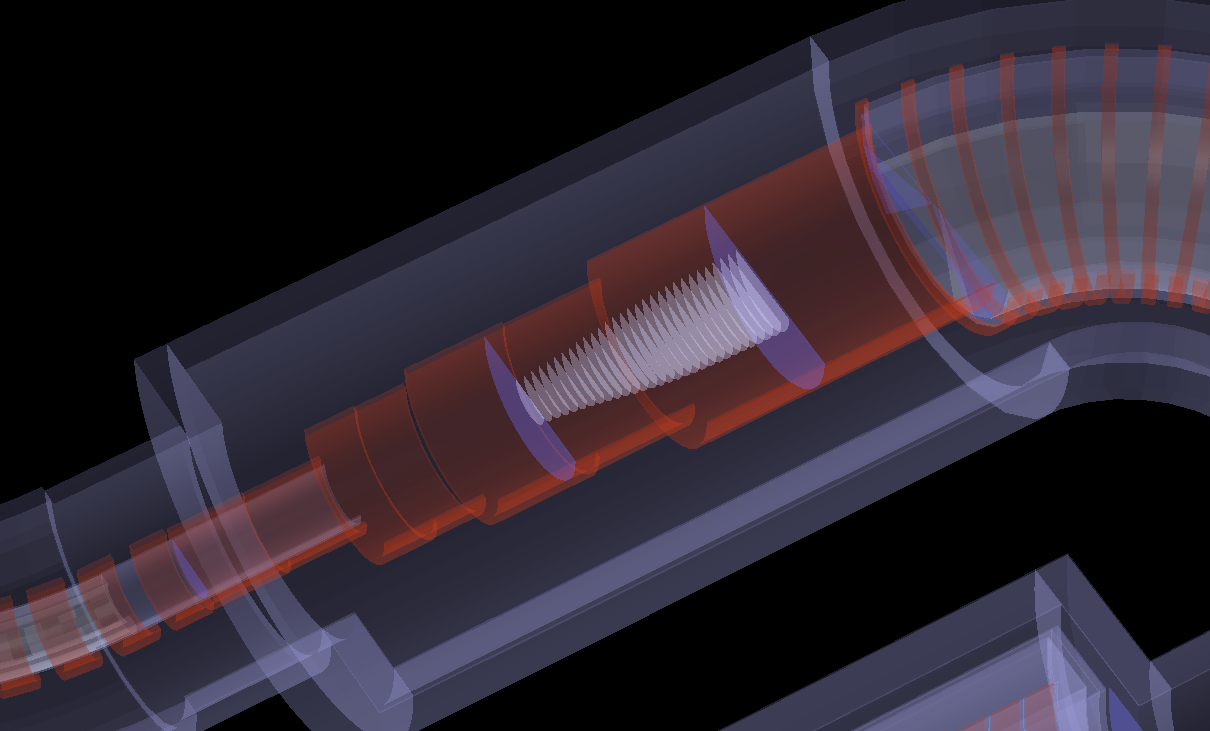
\includegraphics[width=0.7\textwidth]{figs/appendixStopTgtImprov/NewGeometry.png}
\caption{
The new geometry of the stopping target, with the beam blocker removed.
The blue vertical planes are the virtual monitors used in the simulation and not a physical piece of material.
\figlabel{app:tgtImprov:newGeom}}
\end{figure}
}

\newcommand{\FigTgtImprovMuStops}{
\begin{figure}[ptb]
\begin{minipage}[b]{0.35\textwidth}
\subfloat[][\figlabel{app:tgtImprov:muStops:XZ}Above Target (X-Z)]{%
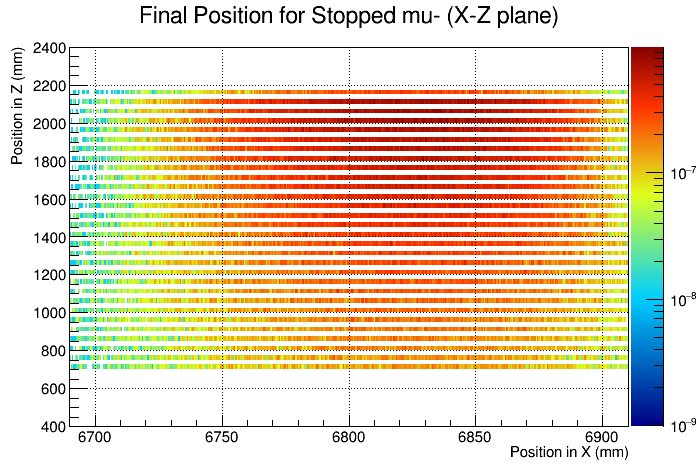
\includegraphics[width=\textwidth,trim=0 0 0 0,clip]{figs/appendixStopTgtImprov/Tidied_Mu_StopPosition_XZ.png}}\\
\subfloat[][\figlabel{app:tgtImprov:muStops:YZ}Side View (Z-Y)]{%
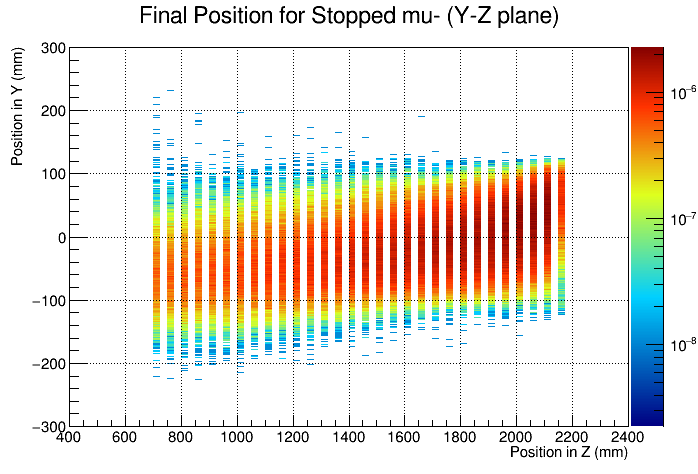
\includegraphics[width=\textwidth,trim=0 0 0 0,clip]{figs/appendixStopTgtImprov/Tidied_Mu_StopPosition_ZY.png}}
\end{minipage}
\subfloat[][\figlabel{app:tgtImprov:muStops:Z}Z Projection]{%
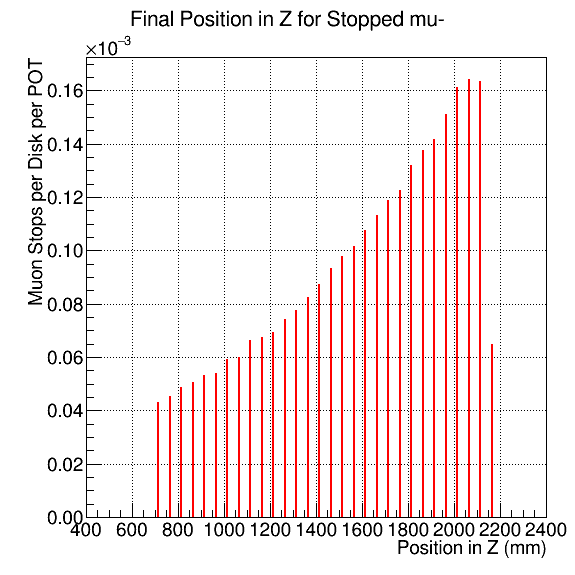
\includegraphics[width=0.5\textwidth,trim=0 0 0 0,clip]{figs/appendixStopTgtImprov/Tidied_Mu_StopPosition_Z.png}}
\caption{
Projections of the muon stopping distribution with the improved target design, to be compared to \fig{sense:stops}.
Although the disks are symmetric, it is clear from \protect\subref{fig:app:tgtImprov:muStops:YZ} how there are fewer muon stops in the upper parts of the disks.
Removing the material there will improve the signal acceptance further.
\figlabel{app:tgtImprov:muStops}}
\end{figure}
}

\newcommand{\FigTgtImprovMuMomentum}{
\begin{figure}[ptb]
\subfloat[][\figlabel{app:tgtImprov:muMomentum:lin}Linear Scale]{%
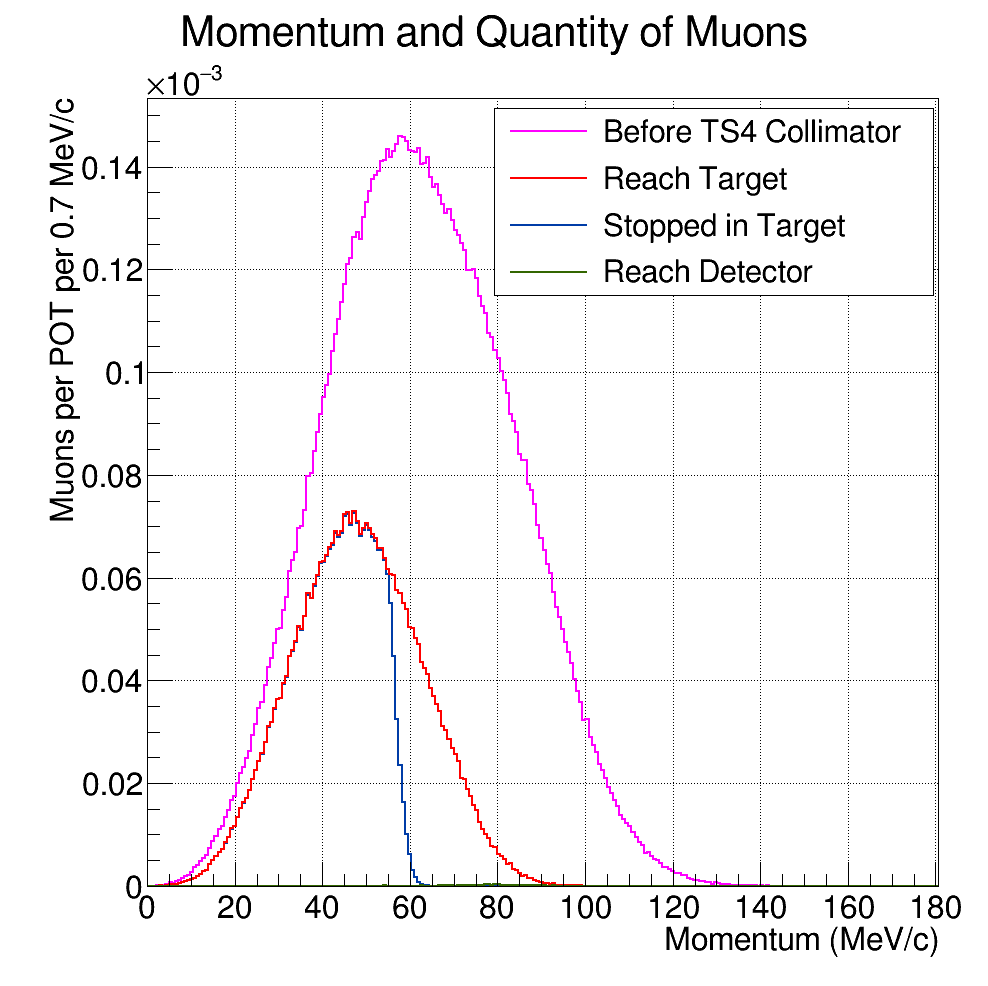
\includegraphics[width=0.49\textwidth,trim=0 0 0 0,clip]{figs/appendixStopTgtImprov/Tidied_muon_momentum_withDetectedMuons_lin.png}}
\subfloat[][\figlabel{app:tgtImprov:muMomentum:log}Logarithmic Scale]{%
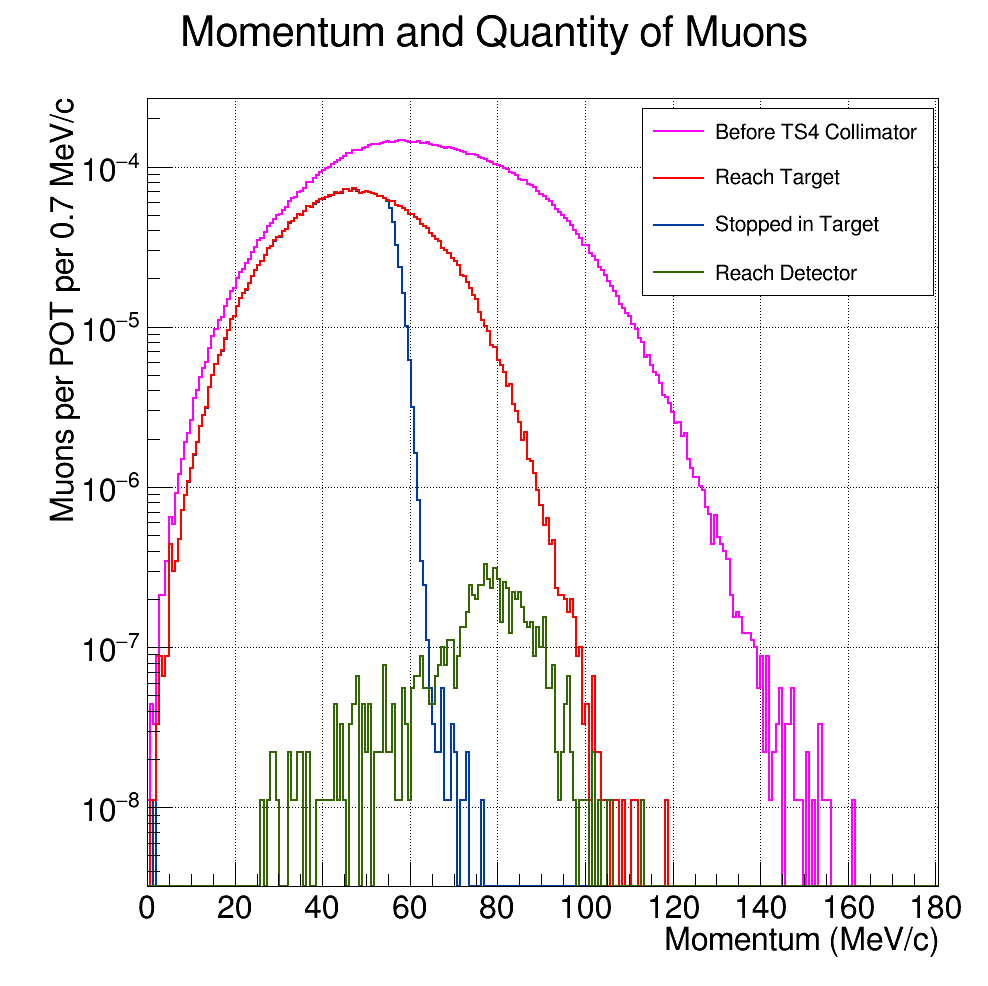
\includegraphics[width=0.49\textwidth,trim=0 0 0 0,clip]{figs/appendixStopTgtImprov/Tidied_muon_momentum_withDetectedMuons_log.png}}
\caption{
The momentum of muons that reach the stopping target and eventually stop.
By comparison with \fig{sense:muMomenta}, the new target design is clearly able to stop much higher momentum muons, although without the beam blocker
it is also clear that high energy muons reach the detector.
\figlabel{app:tgtImprov:muMomentum}}
\end{figure}
}

\newcommand{\FigTgtImprovSignalDistribution}{
\begin{figure}[tb]
\subfloat[][\figlabel{app:tgtImprov:signalMom:lin}Linear Scale]{%
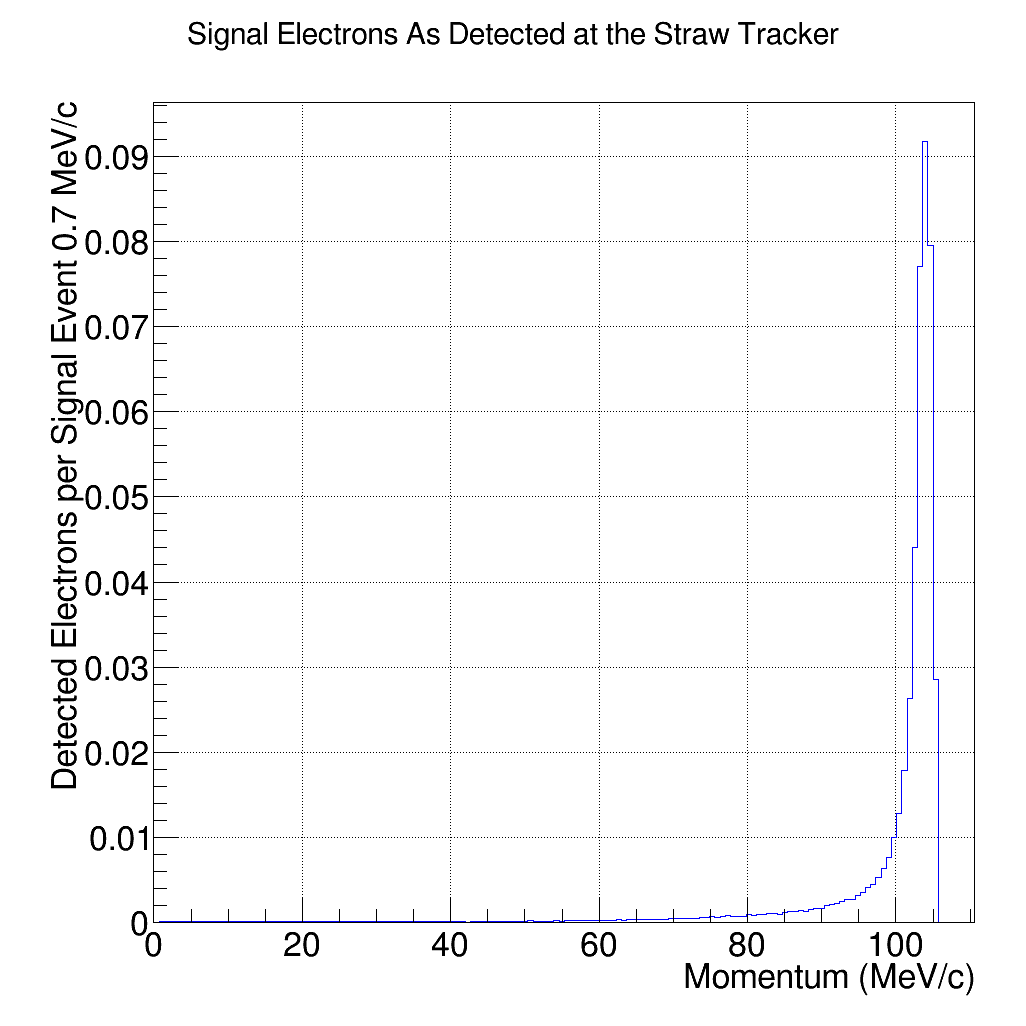
\includegraphics[width=0.49\textwidth,trim=0 0 0 0,clip]{figs/appendixStopTgtImprov/Tidied_StrawTrk_DetectedSignal.png}}
\subfloat[][\figlabel{app:tgtImprov:signalMom:log}Logarithmic Scale]{%
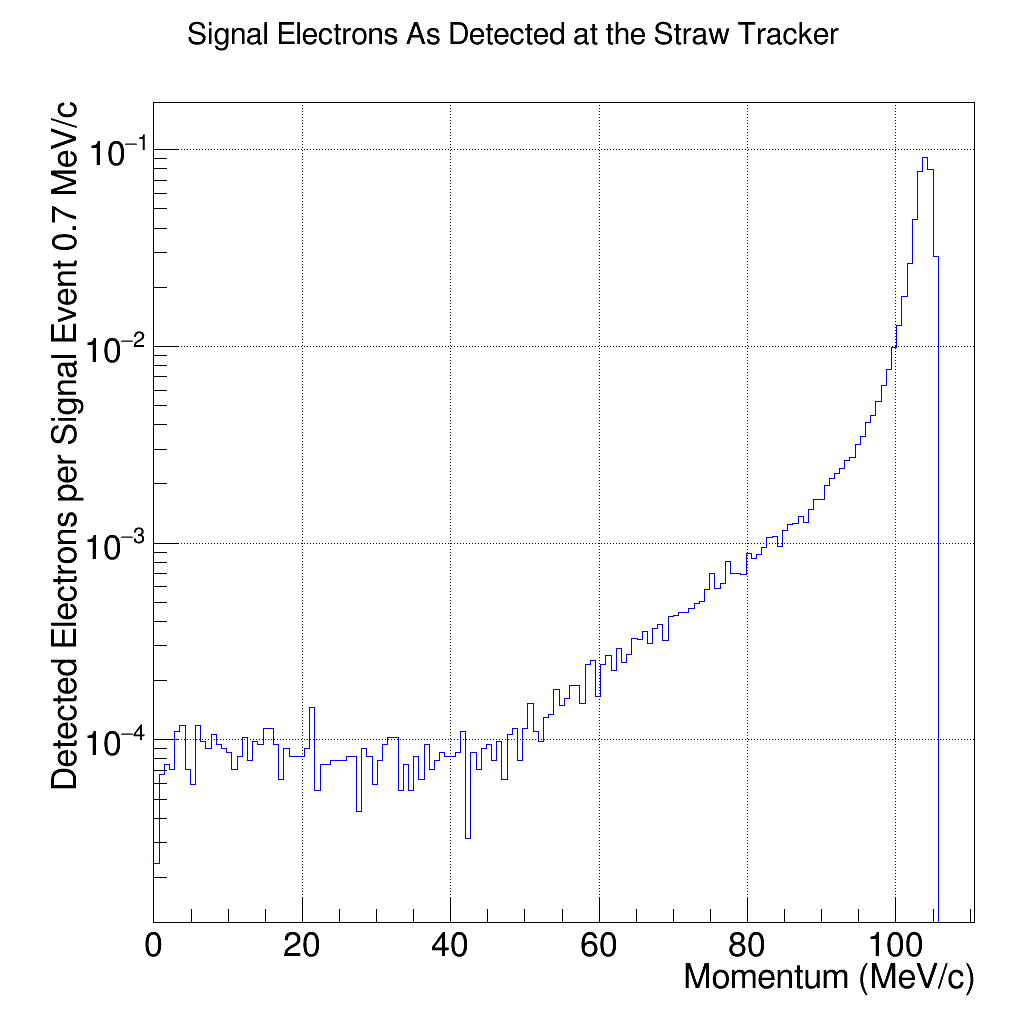
\includegraphics[width=0.49\textwidth,trim=0 0 0 0,clip]{figs/appendixStopTgtImprov/Tidied_StrawTrk_DetectedSignal_log.png}}
\caption{
The observed  momentum distribution and acceptance for signal electrons.
Given the extra material, the energy losses in the target are larger than the previous design, although the overall geometric acceptance is significantly increased.
\figlabel{app:tgtImprov:signalMom}}
\end{figure}
}
